\chapter{Background}
L'obiettivo di questo capitolo è di fornire le conoscenze necessarie per poter comprendere
l’analisi affrontata nei capitoli successivi. Esse comprendono l'introduzione all'analisi di un
segnale (con relativo concetto di spettrogramma), la sua rappresentazione mediante le
caratteristiche selezionate, la standardizzazione dei dati, la classificazione ed infine l’\textit{anomaly
detection}.

\section{Dall’analisi del suono allo spettrogramma}
Il suono nasce dalla vibrazione o oscillazione di un corpo sonoro. Queste vibrazioni creano
delle onde sonore, cioè variazioni di pressione del mezzo che le propaga, per esempio l’aria.

L’onda sonora è definita da tre caratteristiche: l’ampiezza, la frequenza [4] e il timbro [5].

L’ampiezza (o intensità) dell’onda è associata a quanto il suono è percepito intenso (il
volume) ed è misurata in \textit{Decibel}.

La frequenza (o altezza) identifica il numero di oscillazioni in un secondo, esprime un valore
minore o maggiore in base a che il suono risulti più grave o più acuto, determinando così il
tono, ed è calcolata in \textit{Hertz}. La frequenza più bassa è definita come fondamentale e
corrisponde al tono percepito del suono. Oltre alla fondamentale, ogni suono complesso
contiene armoniche, che sono frequenze multiple della fondamentale. L’insieme di queste
frequenze definisce lo spettro del suono che caratterizza un onda sonora.

Il timbro, infine, è la qualità percepita del suono che ci permette di distinguere due strumenti
musicali che stanno eseguendo la stessa nota (quindi stessa frequenza) alla stessa intensità
(stessa ampiezza). Il timbro è influenzato dalla forma dell’onda sonora e dallo spettro.

Nel quotidiano utilizzo del mondo digitale, è comune visualizzare un segnale audio come
un'onda, senza sapere che questa prospettiva rappresenta graficamente l’andamento
dell’ampiezza (sull’asse delle ordinate) in funzione del tempo (l’asse delle ascisse). Questo
tracciato è il risultato di un processo, il campionamento, effettuato sul segnale analogico,
ovvero sulla forma originale del suono rilevato, che trasforma i campioni, ad intervalli
regolari, in segnale digitale. Poiché la struttura digitale non è in grado di cogliere il segnale
originale nella sua forma continua, nella sua reale interezza, il campionamento registra in
forma discreta, ovvero traccia un valore numerico, discreto, a intervalli regolari. Maggiore è
la frequenza di campionamento quindi, il numero di campioni analizzati per ogni secondo,
maggiore è la qualità del risultato. Gli intervalli di campionamento sono come delle
istantanee che misurano e registrano digitalmente il valore dell’ampiezza del segnale in
precisi istanti di tempo.

Il segnale campionato viene rappresentato nel \textit{dominio del tempo}, cioè lo spazio che misura la
variazione dell’ampiezza rispetto al tempo. Questo punto di vista è molto utile per
evidenziare la durata dei suoni, la durata delle pause e la struttura temporale del segnale.
Tuttavia, per poter analizzare nel dettaglio le componenti frequenziali, si deve effettuare un
cambio di prospettiva. Si applica la \textit{Trasformata di Fourier} [7], una funzione in grado di
suddividere l’onda complessa nelle sue sottocomponenti sinusoidali, permettendo quindi di
visualizzare il segnale nel \textit{dominio delle frequenze}, dove l’ampiezza è in rapporto con le
frequenze.

Se invece di eseguire la trasformata sull’intero segnale, lo si suddivide in blocchi, o finestre
temporali, e su ognuna si applica separatamente la funzione, si ottengono più spettri di
frequenza, uno per ogni intervallo. Questi spettri, combinati in un'unica rappresentazione,
formano lo spettrogramma, un grafico che mostra l’andamento delle frequenze in funzione
del tempo. Tale prospettiva ci permette di cogliere in combinazione le informazioni temporali
e frequenziali. In questa processo è importante la dimensione della finestra temporale e del
passo, che definisce quanto si devono sovrapporre le finestre consecutive. Il numero di
campioni analizzati per gruppo determina la dimensione della finestra. Maggiore è il numero
di campioni considerati, minore sarà il numero di finestre utilizzate nel calcolo dello
spettrogramma. Una finestra maggiore determina una migliore risoluzione delle frequenze,
ma una peggiore risoluzione temporale. Il passo, tipicamente, viene impostato ad un valore
uguale alla metà del numero di campioni utilizzati per la finestra.

\begin{figure}[htp] 
	\centering 
	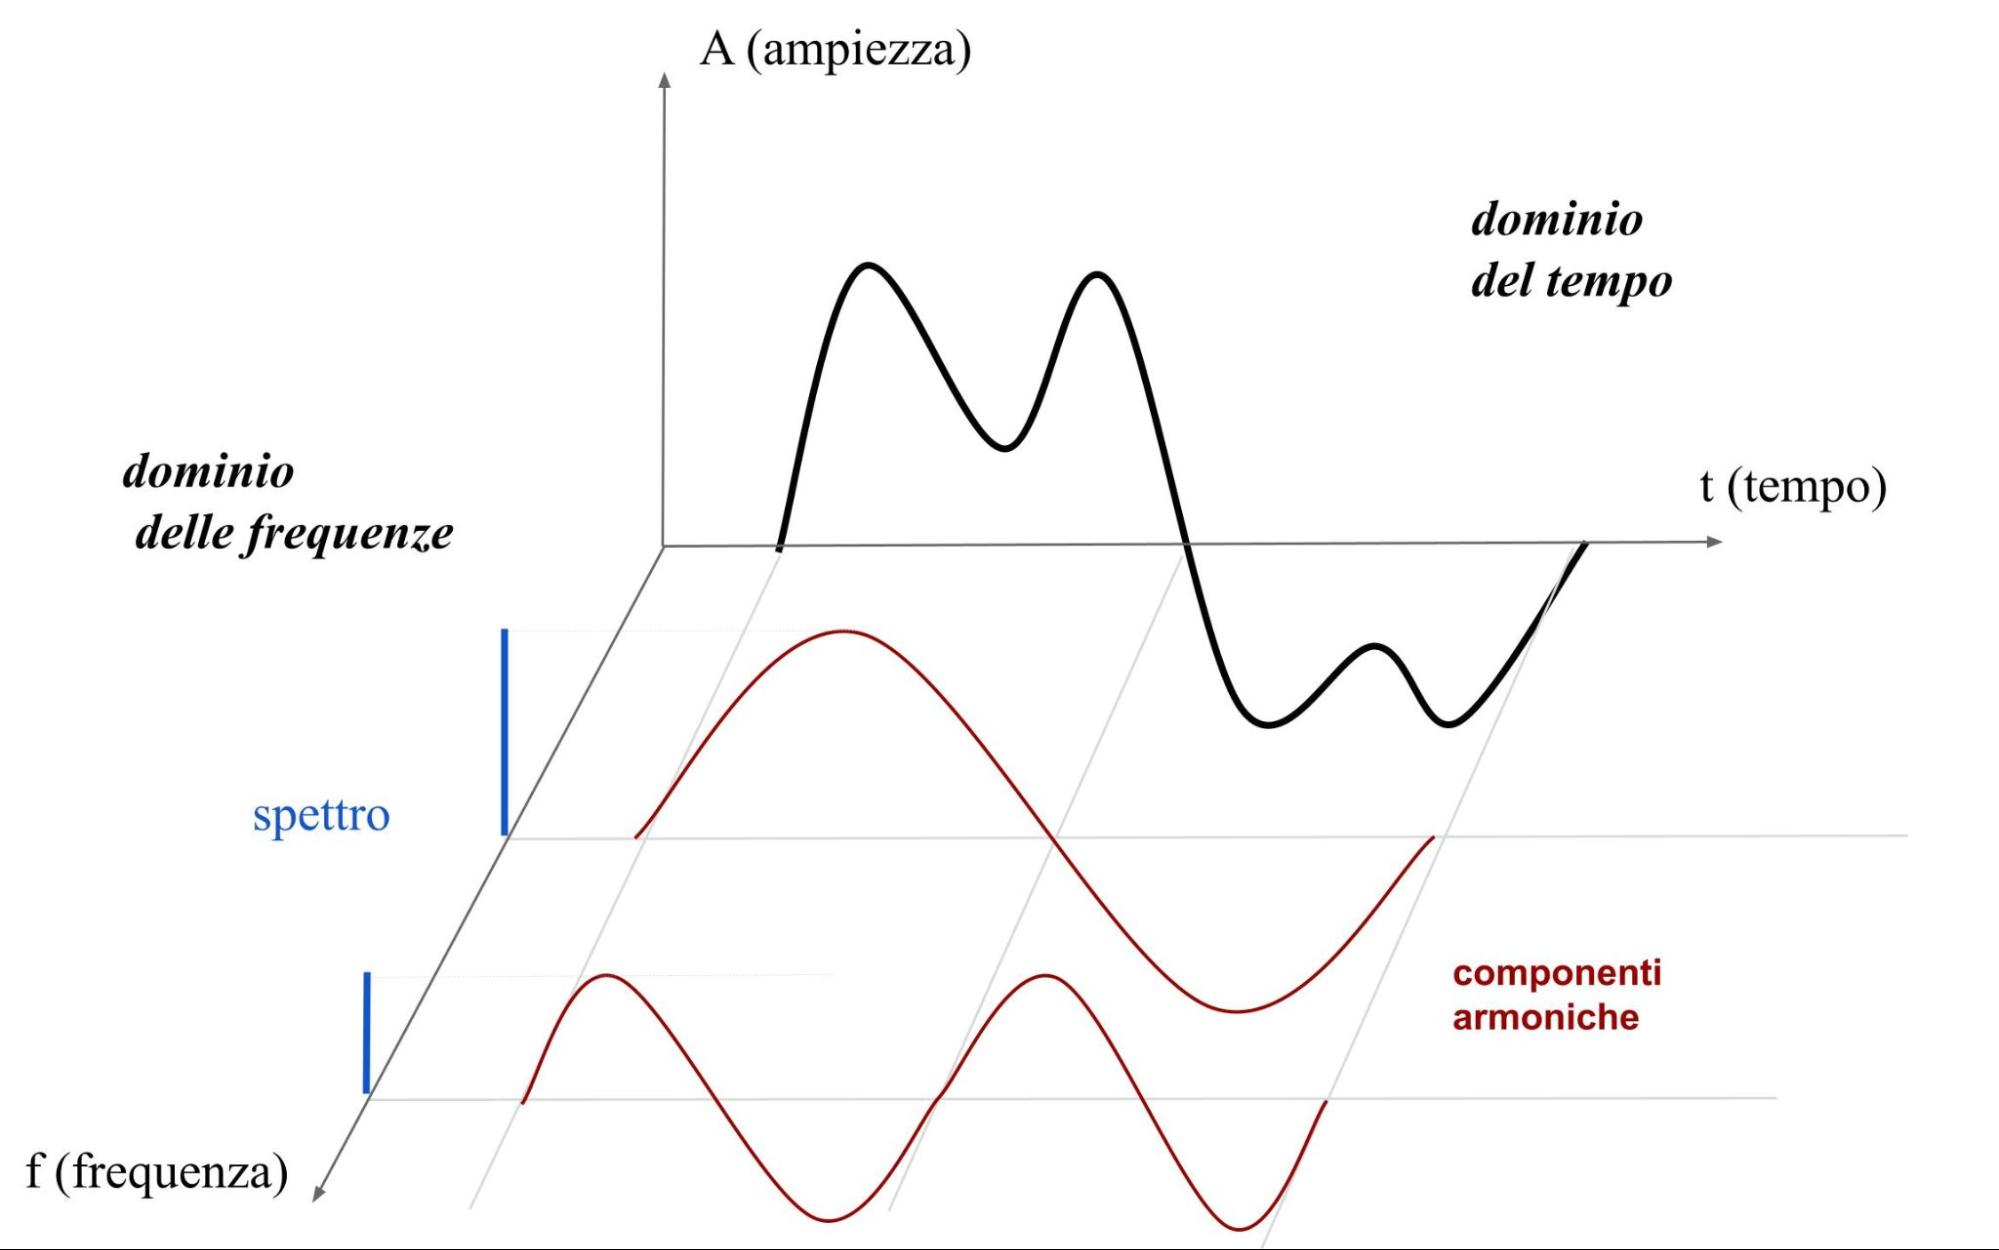
\includegraphics[width=0.9\textwidth]{img/cap2-dominioTempoFrequenza.jpg}
	\caption{Relazione tra dominio del tempo e dominio delle frequenze. In alto a destra la forma d’onda (in nero)
		rappresentata nel dominio del tempo in rapporto al tempo e all’ampiezza. Sotto le varie componenti armoniche
		dell’onda (forme ondulate in rosso). A sinistra viene rappresentato il dominio delle frequenze che presenta le
		ampiezze delle frequenze armoniche di cui è composta l’onda.} 
	\label{fig2.1}
\end{figure}
\begin{figure}[htp]
	\centering
	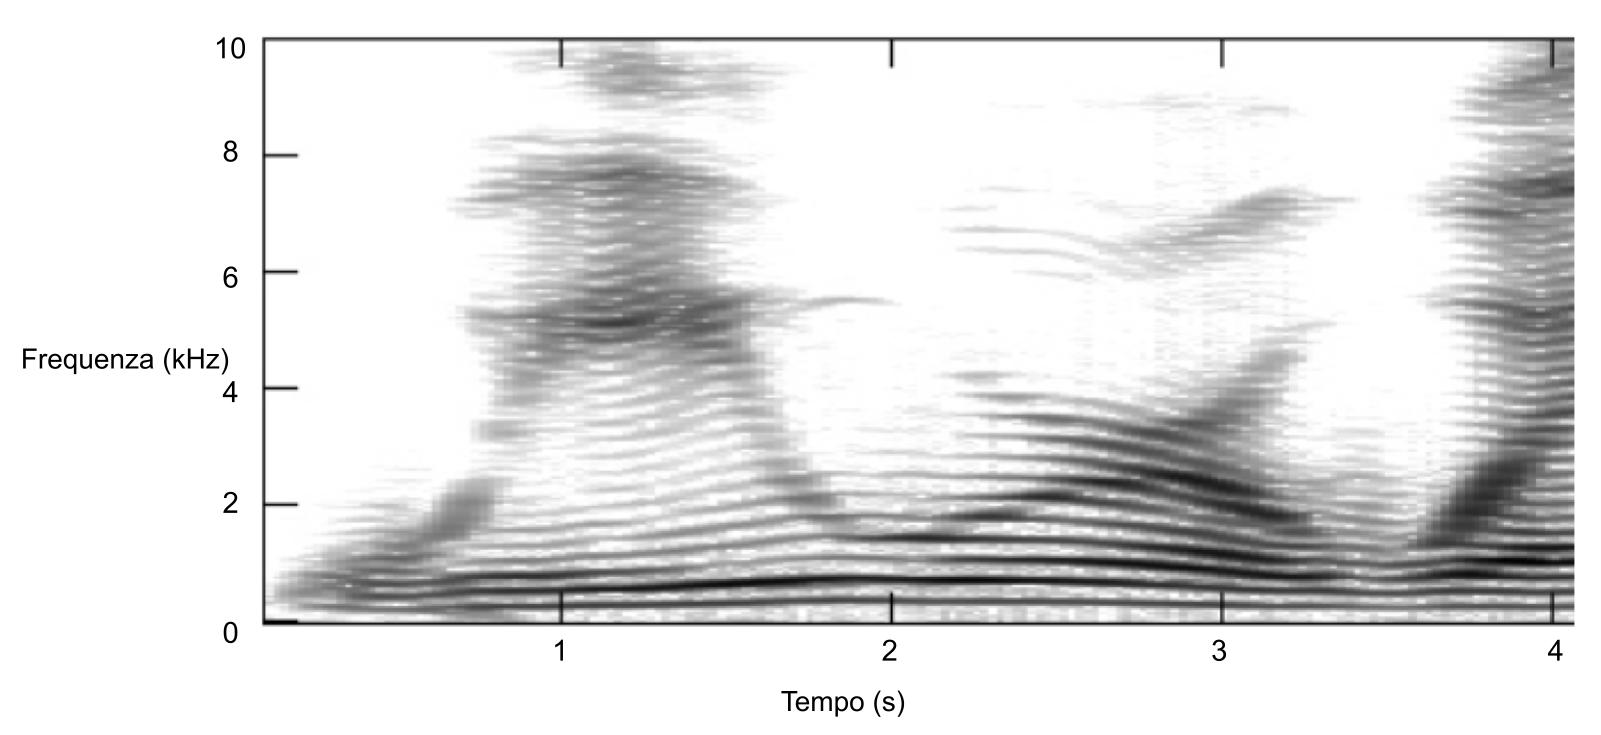
\includegraphics[width=0.9\textwidth]{img/cap2-spettrogramma.jpg}
	\caption{Spettrogramma di un file audio. Tale rappresentazione mostra come varia intensità nel tempo e nella frequenza. La scala di colori va dal bianco, che indica un'intensità sonora bassa, al nero, che rappresenta un'intensità sonora alta}
	\label{fig2.2}
\end{figure}

\clearpage
\section{Estrazione delle \textit{features}}
Distinguere due oggetti qualsiasi, come una bottiglia e una mela, può sembrare una capacità
comune, per nulla speciale. Questa abilità è frutto di un meccanismo che il nostro cervello
sviluppa attraverso l’esperienza e la conoscenza. Per ogni oggetto con cui interagiamo, la
mente elabora un insieme di caratteristiche in grado di descriverlo e lo esegue con una tale
velocità che nemmeno ce ne accorgiamo. Il cervello estrae elementi in grado di definire
l’oggetto, come il colore, la lunghezza e la forma, e con ogni senso del corpo. L’oggetto è da
intendersi anche come un profumo, un suono, un'immagine o qualsiasi altra percezione.

Al fine di insegnare questa capacità ad una macchina, è necessario identificare ciò che è
rilevante, discriminante e misurabile nei dati: le caratteristiche, o \textit{features}. Le \textit{features}
forniscono le informazioni necessarie per costruire il modello in grado di individuare i
\textit{pattern} nei dati e generalizzare, ovvero la capacità di riconoscere anche oggetti mai visti.

In questo studio, che tratta di \textit{soundscape}, l’oggetto da analizzare è un segnale audio. Per
caratterizzare tale segnale sono state utilizzate delle classiche misure di \textit{signal processing},
che si basano sui concetti illustrati nel paragrafo precedente.

Si possono distinguere tre gruppi principali di \textit{features}: spettrali (SPE), tonali (TON) e
temporali (TEM) [7].

Le SPE caratterizzano la forma dello spettro e influenzano le percezione del timbro. Tali
features vengono calcolate sullo spettrogramma del segnale. Si suddividono in:
\begin{itemize}
	\item{\textit{Spectral Centroid}: consiste nella media pesata delle frequenze nel segnale e indica il
		centroide, ovvero il centro di massa dello spettro. Valori più elevati indicano un suono
		più brillante [7]. Per brillante si intende che la maggioranza delle armoniche si trova
		su alte frequenze.}
	\item{\textit{Spectral Spread}: misura la dispersione delle frequenze attorno al centroide [7]. Un
		valore  basso indica una concentrazione maggiore delle frequenze attorno al centroide.}
	\item{\textit{Spectral Rolloff}: misura la frequenza al di sotto della quale si trova una percentuale
		specifica dell'energia totale dello spettro. Valori bassi indicano una scarsa presenza di
		componenti ad alte frequenze [7].}
	\item{\textit{Spectral Decrease}: misura quanto l’energia spettrale cala rapidamente all’aumentare
		delle frequenze. Un curva ripida indica una diminuzione rapida dell’energia spettrale,
		quindi un blocco ricco di basse frequenze e povero di alte frequenze [7].}
	\item{\textit{Spectral Flux}: rileva il numero di cambiamenti nella forma dello spettro. Identifica
		variazioni rapide e significative nel contenuto del segnale [7].}
\end{itemize}
Le TON misurano le componenti tonali del segnale rispetto al rumore. Tali feature vengono
calcolate sullo spettrogramma del segnale. Sono composte da:
\begin{itemize}
	\item{\textit{Spectral Crest Factor}: descrive il rapporto tra il valore massimo delle magnitudini
		dello spettro e la somma di tutte le magnitudini dello spettro (la magnitudo si riferisce
		all’ampiezza massima raggiunta da ogni frequenza nello spettro del segnale). Un
		valore basso indica un segnale molto uniforme [7].}
	\item{\textit{Spectral Flatness}: indica quanto lo spettro è uniforme. Un valore alto suggerisce un
			segnale con poca struttura tonale, quindi molti rumori.}
	\item{\textit{Spectral Tonal Power Ratio}: rapporta l’energia tonale con l’energia totale. Un valore
			alto indica che l’energia si concentra in componenti tonali, basso sui rumori [7].}
\end{itemize}
Infine le TEM, che descrivono come il segnale varia rispetto al tempo. Tali features vengono
calcolate sul segnale nel dominio del tempo. Si suddividono in:
\begin{itemize}
	 \item{\textit{Time Zero Crossing Rate}: identifica il numero di volte in cui il segnale cambia di
	 	segno quindi quando ha valore zero. Un valore alto indica una forte presenza di alte
	 	frequenze [7].}
	 \item{\textit{Time Acf Coeff}: quantifica la correlazione tra il segnale e una versione ritardata dello
	 	stesso (funzione di autocorrelazione). Questa misura è utile per identificare pattern
	 	ripetitivi [7].}
	 \item{\textit{Time Max Acf}: indica il valore massimo dell’autocorrelazione. Un valore alto può
	 	esprimere una forte periodicità del segnale [7].}
\end{itemize}	

\section{Standardizzazione dei dati}
La standardizzazione è un'attività di pre-processamento dei dati in grado di trasformarli in
una forma indipendente dalla scala utilizzata. Per scala si intende l’intervallo in cui le varie
\textit{features} vivono, ed è fondamentale per confrontare i dati. Infatti, una certa misurazione può
avere un rapporto diverso con gli altri dati a seconda della scala. Immaginiamo di avere i
risultati di due esami scolastici diversi, fatti da due gruppi di studenti. Il primo gruppo ha
ottenuto i risultati in centesimi, un intervallo da 1 a 100, invece il secondo gruppo, in
trentesimi, da 1 a 30. Un voto di 30 nel primo gruppo è molto diverso da un voto 30 nel
secondo gruppo: senza standardizzare la scala il confronto è falsato. Si deve quindi riportare
alla stessa scala. La standardizzazione è un insieme di tecniche dove vengono uniformate le
versioni ottenendo una versione standard dei dati, “senza dimensionalità”.

Una tecnica di standardizzazione molto utilizzata è lo \textit{Z-score standardization}, qui specificata
con la formula:
\begin{equation}
	x^{*}_{ji} = \frac{x_{ji} - \overline{x}_{j}}{\sigma_{j}}
\end{equation}
Si definisce \( x^{*}_{ji} \) la \textit{j}-esima \textit{feature} dell’oggetto \textit{i} standardizzata, 
\( x_{ji} \) la \textit{j}-esima feature dell’oggetto \textit{i} prima della standardizzazione, 
\( \overline{x}_{j} \) la media della \textit{feature} \textit{j} ed infine \( \sigma_{j} \) la 
deviazione standard delle \textit{features}. Si consideri ora una matrice composta sulle righe dagli
oggetti in esame e in colonna i valori delle \textit{feature}. Per ogni elemento \textit{x} in riga \textit{j} e posizione \textit{i} viene sottratta la media calcolata in colonna \textit{j}, e il valore ottenuto si divide con la deviazione
standard estratta dalla colonna \textit{j}. Dopo la standardizzazione ogni feature ha media uguale a 0
e deviazione standard a 1.

\section{Classificazione}
La classificazione è uno dei \textit{task} più utilizzati, affrontato con tecniche di PR e ML. Un
classificatore rappresenta un sistema decisionale in grado di assegnare una categoria, o
etichetta, ad un oggetto sulla base di un modello, tipicamente a partire da una descrizione
vettoriale (vettore di \textit{features}). In sostanza, è una funzione che prende in input un oggetto, ne
elabora le \textit{features} e restituisce un valore discreto che determina a quale categoria appartiene.

In generale gli approcci alla classificazione si suddividono in generativi e discriminativi.

Nell’approccio generativo si mira a definire un modello per ogni categoria, o classe. Questa
tipologia di approcci presenta una struttura più flessibile in grado di adattarsi a nuove classi, è
più rapida nell’addestramento e ottiene una migliore capacità descrittiva per la singola classe.

L’approccio discriminativo, invece, si basa sulla ricerca del migliore confine decisionale per
separare le classi nello spazio. Per sua natura è più rapido, soprattutto nella fase di test, e
presenta un'efficacia di classificazione migliore dato che il sistema viene costruito
specificatamente per risolvere il problema di classificazione.

Un'ulteriore suddivisione nei classificatori si basa sulla loro natura parametrica o non
parametrica. La parametrica si caratterizza per l’assunzione della forma di distribuzione dei
dati per ogni classe (es. la distribuzione normale), e si concentra nella stima dei parametri
della funzione che genera tale distribuzione. Diversamente, la non parametrica non assume
nessuna forma di distribuzione, ma viene stimata direttamente dal \textit{training set}. Risulta più
dispendiosa in termini computazionali ma non basandosi su assunzioni determina un modello
maggiormente flessibile e adattabile al contesto.

\subsection{Apprendimento supervisionato}
Nella PR spesso si utilizza il paradigma dell’\textit{apprendimento da esempi}. Questo metodo può
essere visto come l’apprendimento di un bambino che sperimenta e acquisisce conoscenza da
esempi, dall’esperienza. In particolare, nel contesto della classificazione, si utilizza un
approccio supervisionato in cui la conoscenza viene acquisita tramite dati campionati dal
problema, il \textit{training set}, dotato di categorie, o etichette, note. Conoscendo la reale classe di
appartenenza degli oggetti, il modello può addestrarsi e migliorare gradualmente la sua
capacità di classificazione. In questo processo è importante che il sistema non “impari a
memoria” i dati del \textit{training set}, il cosiddetto \textit{overfitting}, che comporta un eccessivo
adattamento ai dati di addestramento. L’obiettivo infatti è di creare un modello in grado di
generalizzare quindi di classificare correttamente anche oggetti sconosciuti, mai visti.

\subsection{Validazione}
Una volta costruito il modello è necessario verificare la qualità del classificatore. Per tale
scopo si utilizza il \textit{testing set}, un \textit{dataset} che presenta elementi diversi da quelli usati in
addestramento, ma dotato di categorie note da confrontare con il risultato predetto dal
classificatore. Il modello classifica tali dati e si valuta la predizione in base all’errore
ottenuto. Questo valore pone in rapporto le previsioni errate rispetto al numero totale di
oggetti analizzati. Una previsione errata consiste in una falsa valutazione del classificatore,
quindi un valore diverso dalla reale categoria di appartenenza.

Nella costruzione di un classificatore di solito si dispone di un unico \textit{dataset} che si deve
suddividere in due parti, il \textit{training set}, per l’addestramento, e il \textit{testing set} per i test e la
validazione. Un metodo ideale sarebbe poter usare tutti dati di esempio per il \textit{training} ed
estrarre altri esempi dal problema per testare il modello, ma nella realtà potrebbe essere non
fattibile o troppo dispendioso. Si preferisce quindi usare una metodica comune che consiste
nella \textit{cross validation}, che permette di ottenere una valutazione più valida e consistente.
Esistono diverse varianti, ognuna con le sue caratteristiche. La forma più semplice è la
\textit{Holdout}, che distribuisce casualmente i dati in due insiemi di uguale dimensione.
Un'alternativa simile è l’\textit{Average Holdout}, che per essere indipendente dalle partizioni effettua
più \textit{holdout} e calcola l’errore come media dei risultati ottenuti in tutti i casi.

Infine, una delle più utilizzate è la \textit{Leave One Out} (LOO), una variante particolare che ottiene
ottimi risultati in termini di affidabilità, soprattutto con dataset ristretti. Come suggerisce il
nome, consiste nell’effettuare l’addestramento con tutti gli oggetti del \textit{dataset} meno uno, 
\( x_{i} \), che viene invece utilizzato per validare il modello. Si ripete il procedimento lasciando fuori
come oggetto di testing un diverso elemento \( x_{i} \) del \textit{dataset}, e al termine si media il risultato
ottenuto. Presenta un costo computazionale maggiore ma garantisce indipendenza dalla
partizione e dai dati scelti del \textit{training set} e \textit{testing set}.

\subsection{Metodo di classificazione}
In questo studio è stato utilizzato il classificatore \textit{K Nearest Neighbor} (KNN), un approccio
supervisionato generativo non parametrico, semplice e intuitivo: il metodo si basa sul
classificare un punto, un oggetto, assegnandogli la classe che più frequentemente ritroviamo
tra i \textit{k} oggetti più vicini. Il concetto di vicinanza si concretizza con la scelta della distanza: nel
nostro caso la \textit{distanza euclidea}, una delle misure più utilizzate. Come risulta chiaro, la scelta
del valore di \textit{k} è cruciale.


\section{Anomaly Detection}
L’\textit{anomaly detection} (AD) consiste nell’identificare fenomeni ed eventi che presentano un
comportamento anomalo rispetto al resto del \textit{dataset} [8]. Tali fenomeni, denominati \textit{outlier}, si discostano in modo significativo dagli \textit{inlier}, il resto dei dati normali, per la loro natura anomala e la scarsa numerosità.

\begin{figure}[htp]
	\centering
	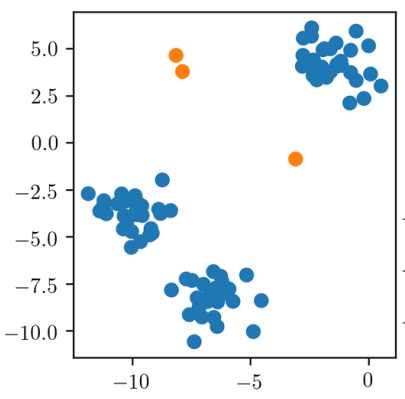
\includegraphics[width=0.4\textwidth]{img/cap2-AnomalyDetection.png}
	\caption{Rappresentazione di \textit{inliers} (cerchi colore blu) e outliers (cerchi colore giallo) in un \textit{dataset}. Si nota come gli \textit{outlier}, in questo caso, risultano distaccati dal comportamento generale definito dagli inlier, che sono raggruppati e seguono una distribuzione più omogenea.}
	\label{fig2.3}
\end{figure}

\subsection{Gli \textit{outlier}}
Individuare gli \textit{outlier}, pur essendo complicato, è una necessità. Ciò consentirebbe di inferire
informazioni preziose oppure rappresentare una prevenzione per eventuali criticità.
Contribuisce in modo significativo anche al data cleaning, la “pulizia dei dati”, che conta di
un insieme di processi che servono a rimuovere duplicati, uniformare e filtrare i dati. In
questo contesto rimuovere gli outlier semplificherebbe le fasi successive di analisi
migliorando la qualità del risultato.

Si distinguono varie tipologie di \textit{outlier}:
\begin{itemize}
	\item{i \textit{point}, che sono identificati tali indipendentemente se si trovano da soli o in gruppo;}
	\item{i \textit{collective}, considerati outlier solo se rilevati in gruppo, altrimenti rientrano negli \textit{inlier};}
	\item{i \textit{contextual}, che sono rilevati normali o anomali in base al contesto specifico in cui si
	trovano. Per esempio, in un sistema di monitoraggio della temperatura di una città,
	una valore di 30 gradi durante l’estate verrà considerato normale, diversamente lo
	stesso valore in inverno sarà definito anomalo.}
\end{itemize}

\subsection{Le applicazioni}
L’AD ricopre un ruolo importante in molteplici campi. Per esempio, possiamo citare:
\begin{itemize}
	\item{le intrusioni di rete: in un rete informatica di sistemi che condividono informazioni
	monitorare attività sospette o non autorizzate è fondamentale. Tali attività, come un
	programma o un individuo malevole, potrebbero insinuarsi con lo scopo di rubare dati
	o compromettere la sicurezza. Sistemi basati su AD consentono di rilevare tali
	comportamenti come anomali poiché si discostano dal traffico della rete considerato
	normale;}
	\item{l’ambito sanitario: fondamentale nell’analisi dei dati dei pazienti per diverse ragioni
	come condizioni di salute anomale, errori nella strumentazione o nelle registrazioni
	mediche. Tale approccio potrebbe contribuire in modo significativo nel rilevamento di
	situazioni potenzialmente critiche, sia per intervenire in anticipo che per evitare errori
	nella diagnosi;}
	\item{i sistemi automatizzati, in cui prevenire un avaria o, riuscire a intervenire in tempo nel
	caso si manifestasse, è essenziale;}
	\item{nel processamento di immagini o testi, come rilevare \textit{fake news};}
	\item{nel rilevamento di frodi, all’interno delle innumerevoli transazioni bancarie prodotte
	ogni giorno.}
\end{itemize}
Queste casistiche sono accomunate da un enorme quantità di dati dove sistemi troppo rigidi e
specifici non potrebbero adattarsi al continuo mutamento delle variabili in gioco. Le
problematiche nell’AD sono svariate. I contesti affrontati non sono supervisionati, non vi è
modo di basarsi su esempi espliciti di \textit{outliers} dato che non esiste una chiara definizione di
ciò che rende un'anomalia tale e il rischio di determinare falsi positivi è molto alto.

\subsection{I metodi}
I diversi approcci di AD tipicamente si suddividono sulla base del metodo utilizzato per
rilevare le anomalie. I vari metodi possono essere:
\begin{itemize}
	\item{Metodi basati sui concetti statistici: essi ricercano elementi che non rispecchiano la
		distribuzione dei dati. Una bassa probabilità di appartenenza alla distribuzione
		determina un'alta probabilità di essere un \textit{outlier}.}
	\item{Metodi basati sul \textit{clustering}: essi suddividono i dati per somiglianza in gruppi, i
		cluster, e le anomalie risultano evidenti poiché molto diverse dal loro gruppo di
		appartenenza. Oppure gli \textit{outlier} formano piccoli cluster che presentano una
		dimensione o una densità inferiori alla soglia necessaria per essere considerati tra i
		dati normali, venendo quindi identificati come anomalie.}
	\item{Metodi basati sull’apprendimento: vengono utilizzati metodi di apprendimento
		automatico per ricercare \textit{pattern} all’interno dei dati. Gli elementi che non si
		identificano in questi \textit{pattern} vengono considerati come anomalie.}
	\item{Metodi basati sulla distanza o sulla densità: viene considerata la distanza tra gli
		elementi, o la densità locale. Nel primo caso gli \textit{outlier} si troveranno distanti dagli
		altri punti, nel secondo saranno in zone a bassa densità.}
	\item{Metodi basati sulla combinazione di vari metodi, o \textit{ensemble}: queste tipologie
		combinano i risultati di metodi diversi, o gli stessi con parametri differenti, per
		ottenere una previsione più accurata.}
\end{itemize}	
La maggioranza degli algoritmi ritorna come risultato un valore, denominato \textit{Anomaly score},
che quantifica quanto un elemento è probabile che sia un’anomalia.

In letteratura esistono differenti algoritmi di AD [8], ma di seguito ne saranno descritti solo
tre, quelli utilizzati nello studio. I metodi sono L’\textit{IForest} (IF) [9], o \textit{Isolation forest}, il \textit{Local Outlier Factor} (LOF) [10] e l’\textit{Ocsvm} (OCSVM) [11], o \textit{One Class Support Vector Machine}.

IF è un algoritmo basato su un \textit{ensemble} [8] di alberi decisionali. Per albero decisionale si
intende una struttura ad albero dove ogni nodo contiene un test e i rami le possibili risposte.
Procedendo dall’alto verso il basso del modello, i dati vengono indirizzati dalle varie risposte
fino alle foglie, lungo il path. In IF viene costruita una foresta di alberi decisionali e ciascun
albero cerca di isolare i dati mediante suddivisione. L’idea è che le anomalie avranno un path
più corto poiché avranno bisogno di meno divisioni rispetto ai dati normali. In sostanza, più
risulta facile isolare un oggetto e con maggiore probabilità sarà un anomalia. Questo
algoritmo risulta molto scalabile, veloce e accurato, specialmente su dataset di grandi
dimensioni.

LOF è un metodo basato sulla densità. La densità di un oggetto può essere calcolata
guardando al suo vicinato, ovvero dalla numerosità degli elementi che gli sono vicini. Il
criterio utilizzato per determinare la vicinanza ad un oggetto dipende dalla metrica scelta
nell’implementazione. La più comune è la distanza euclidea, che misura la lunghezza del
segmento tracciato tra due punti. In sostanza, l’algoritmo stabilisce che minore è la densità
locale allora più alta è la probabilità che un determinato oggetto possa essere un’anomalia.
Questo metodo è efficace con dati ad alta dimensionalità, ma al contrario, risulta molto
dispendioso in termini computazionali.

Infine, OCSVM si basa sull’apprendimento. Si tratta di una variante delle \textit{Support Vector Machine}, un approccio discriminativo applicato solitamente a problemi binari. In questa
forma, a singola classe, l’algoritmo viene addestrato per definire un confine che racchiude al
suo interno solo i dati normali. Così facendo i dati anomali, che risultano esterni alla
distribuzione, emergono e sono quindi rilevabili. Spesso viene utilizzato il trucco del \textit{kernel},
che consiste nel proiettare i dati in una dimensione superiore, dove può risultare più facile
separare i dati.